% !TEX root = Thesis.tex

%==============================================================================
\chapter{Erbium \acl*{bec}}
\label{chap:erbium_bec}
%==============================================================================

This chapter has the objective of briefly review some relevant properties of Erbium, which will clarify what makes it relevant in the study of ultra cold atoms. After this, the basic theory of Bose-Einstein condensation will be discussed, along with a brief description of the experimental phases required to create and observe an erbium \ac{bec}. This experimental realization will be the foundation on which the following chapters will be grounded when discussing further experimental achievements.

%==============================================================================
\section{Properties of erbium} \label{sec:erbium_properties}
%==============================================================================
Erbium is a chemical element with an atomic number of 68, which belongs to the series of the Lanthanides. It is also part of the group called Rare-earth elements and it was first discovered by G. Monsander in 1843 \cite{mosander1843xxx}. The name of ``Erbium'' comes from the name of the Swedish village of Ytterby, the place where it was extracted. At that time, the similarity of rare-earth metals' chemical properties made their distinction extremely difficult. For this reason, what G. Monsander thought to be pure Erbium oxide was in fact a mixture of different rare-earth metal oxides. The element is not obtained in a reasonably pure form until 1937 by W. Klemm and H. Bommer \cite{klemm1937bommer}.

Considering some basic properties of this element, under standard conditions erbium is in a solid state. It has a silver shining surface, which oxidizes with air contact. This rare-earth metal has a melting point of \SI{1802}{\kelvin} and boiling point of \SI{3136}{\kelvin}. As a result, to be able to work with a free atomic gas of erbium requires to heap up the solid erbium metal to high temperatures \cite{emsley1998}.

The number of stables isotopes of Erbium is 6 and they can be seen in Table \ref{tab:Isotopes_Erbium}. All of them are bosons with nuclear spin of zero, in exception of $^{\text{167}}\text{Er}$, which is a fermion with spin of 7/2. The chosen isotope for this experiment is $^{\text{168}}\text{Er}$ because of its bosonic nature (see Section \ref{sec:bose-einstein_condensation}), high abundance and favorable scattering properties.

\begin{table}[htbp] \centering
	\begin{tabular}{@{}c|c|c|c@{}}\hline
		Isotope                  & Abundance [\%]          & Atomic Mass [u] & Nuclear Spin [$\hbar$] \\ \hline\hline
		$\text{Er}^{\text{162}}$ &  0.14                   & 161.928775      & 0   \\
		$\text{Er}^{\text{164}}$ &  1.61                   & 163.929198      & 0   \\ 
		$\text{Er}^{\text{166}}$ & 33.60                   & 165.930290      & 0   \\
		$\text{Er}^{\text{167}}$ & 22.95                   & 166.932046      & 7/2   \\
		$\text{Er}^{\text{168}}$ & 26.80                   & 167.932368      & 0   \\  
		$\text{Er}^{\text{170}}$ & 14.90                   & 169.935461      & 0   \\  \hline
	\end{tabular}
	\caption[Table with the stable isotopes of Erbium]{Table with the stable isotopes of Erbium that can be found on Nature with their respective Abundance ratio, Atomic mass and Nuclear Spin. Spectroscopy data taken from \cite{sansonetti2005handbook}.}\label{tab:Isotopes_Erbium}
\end{table}

In addition to these properties, erbium atoms have a rather complex energetic level scheme due to its open 4f shell. This one lacks 2 electrons to be completely filled, which makes erbium to have an electronic ground state with an orbital angular momentum value of $L = 5$ and a high magnetic moment of seven Bohr magneton $7\mu_B$ \cite{ban2005laser}. This high value for the orbital angular momentum in the ground state of erbium provides several advantages for Raman-coupling processes. Leading to longer coherence times and stronger synthetic magnetic fields when comparing with other alkali metals like rubidium or cesium, commonly used in ultracold atoms experiments  \cite{cui2013synthetic}.


A scheme of erbium energy levels together with the atomic transitions used in this experiment can be seen in figure \ref{fig:erbium_scheme}. The scheme shows that the electronic ground state of erbium is $\text{[Xe] }\text{4f}^{12} \text{6s}^2$, where [Xe]
represents the complete electronic configuration of Xenon\footnote{$\text{[Xe] = }\text{1s}^2 \text{ 2s}^2 \text{ 2p}^6 \text{ 3s}^2 \text{ 3p}^6 \text{ 3d}^{10} \text{ 4s}^2 \text{ 4p}^6 \text{ 4d}^{10} \text{ 5s}^2 \text{ 5p}^6$}. Moreover, the used optical transitions are represented by colored arrows in the figure and its spectroscopic data is shown in table \ref{tab:Transitions}. From now on, these three transitions will respectively be referred to as the 401nm, 583nm, and 841nm transitions.

Finally, it must be noted that aside from the discussed application in ultracold atoms, erbium is used in multiple commercial applications. One prominent example is the use or erbium as a fiber amplifier in doped silicon fibers \cite{mears1987low}. Furthermore, in nuclear physics it is used as neutron absorbing control rods \cite{emsley2011nature}.

%\sisetup{per-mode = symbol}%

\begin{table}[htbp] \centering
	\begin{tabular}{@{}l|c|c|S|S|S@{}}\hline
		\multicolumn{3}{c|}{Parameters} & \multicolumn{3}{c}{Transitions} \\ \hline
		Name & Symbol & Unit & \multicolumn{1}{c|}{401nm} & \multicolumn{1}{c|}{583nm} & \multicolumn{1}{c}{841nm} \\ \hline\hline
		Wavelength in vacuum & $\lambda$	& \si{\nano\meter}					& 400.91		& 582.84		& 841.22\\
		Lifetime 			& $\tau$	& \si{\micro\second}				& 0.045			& 0.857			& 20   \\ 
		Natural linewidth 	& $\Delta \nu_0$	& \si{\kilo\hertz}					& \num{33370} 	& 185.71 		& 7.96   \\
		Decay rate 			& $\gamma$	& \si{\per\second}					& \num{2.22e8} 	& \num{1.17e6}  & \num{5.00e4} \\
		Saturation intensity & $I_{S}$	& \si{\milli\watt\per\centi\meter}	& 71.80			& 0.12			& 1.74  \\  
		Doppler temperature	& $T_D$	& \si{\micro\kelvin} 				& 848.69  		& 4.46  		& 0.19    \\  
		Doppler velocity	& $v_D$	& \si{\centi\meter\per\second}		& 21.5 			& 1.49 			& 0.31 \\
		Recoil temperature	& $T_R$	& \si{\nano\kelvin} 				& 354.95  		& 167.94  		& 80.43    \\  
		Recoil velocity	& $v_R$	& \si{\milli\meter\per\second}		& 5.93 			& 4.08 			& 2.82 \\  \hline
	\end{tabular}
	\caption[Spectroscopic data for the optical transitions of Erbium]{Spectroscopic data for the optical transitions of Erbium used in this experiment. These transitions are called the 401nm, 583nm, and 841nm transitions and can be seen in figure \ref{fig:erbium_scheme}. Shown spectroscopic data taken from \cite{mcclelland2006natural, lawler2010atomic, den2010radiative, ban2005laser, lipert1993isotope}}\label{tab:Transitions}
\end{table}


\pagebreak


\begin{figure}[!htbp]\centering
	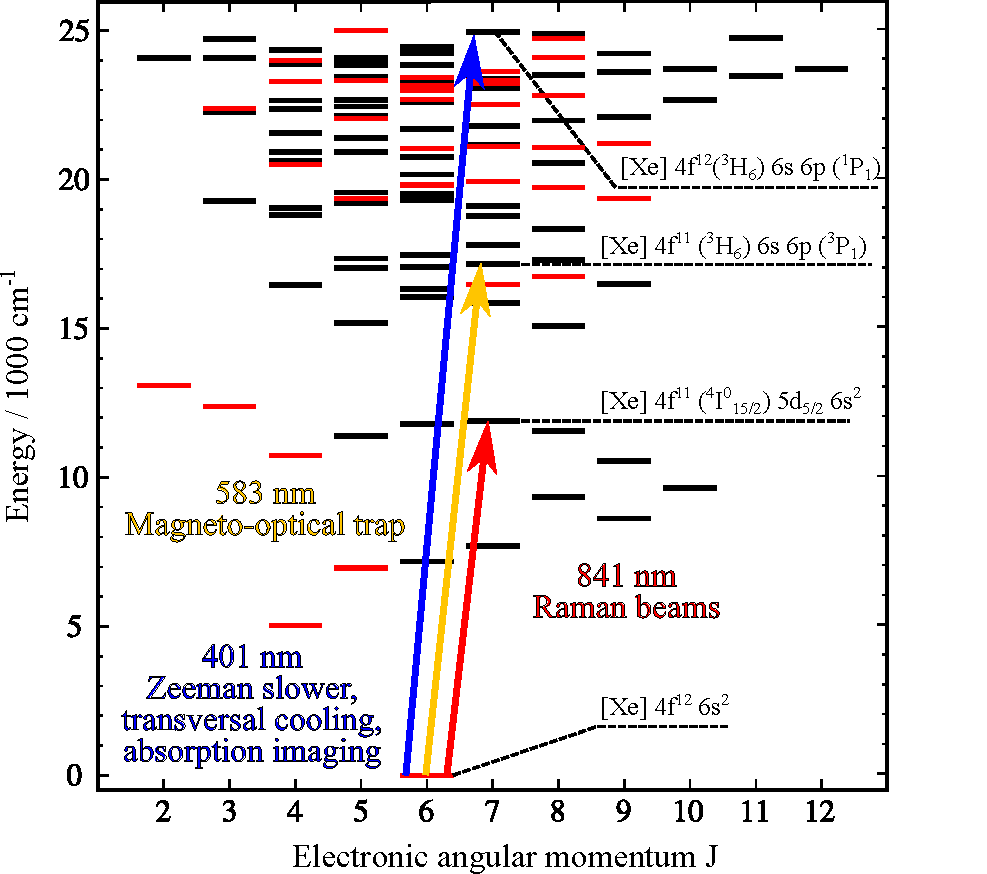
\includegraphics[width=1.\columnwidth]{erbium_term_scheme.pdf}
	\caption[Erbium energy scheme]{Energy level scheme of Erbium represented as a function of the total angular momentum J. This scheme shows only a range of energies relevant for the experiment of up to 25000 $\text{cm}^{\text{-1}}$. The different arrows show us the used transitions and for which phase of the experiment they are used for. The red lines represent energy states with even parity and the black lines those with odd parity. Data taken from \cite{NIST}. }\label{fig:erbium_scheme}
\end{figure}


%==============================================================================
\section{Bose-Einstein Condensation} \label{sec:bose-einstein_condensation}
%==============================================================================

A \ac{bec} is generally defined as a state of matter formed when a gas of bosons with a low density is cooled to near-zero temperatures (typically a few hundreds nanokelvins). To understand this definition and the next theoretical principles is necessary to define what is a Boson. In quantum mechanics, bosons are particles with an integer value in their spin. Because of this,  also have a symmetric wave function under the interchange of two particles, which allows bosons to have the same quantum state. Unlike its counterpart fermions, which have a half odd integer spin and an anti-symmetric wave function. Leading to Pauli's exclusion principle that avoids more than one fermion to occupy the same quantum state \cite{Pauli1925}.

It was the Indian physicist S. N. Bose in 1924, the first one who described in a successful way an ideal gas of non interacting free photons, behaving like mass-less bosons. His idea was initially rejected for publication in scientific journals. However, Bose sent the manuscript to A. Einstein, who recognized its importance, translated the paper to german and saw to it that was published \cite{Bose1924}. After this, Einstein extended Bose's treatment to massive particles and predicted the occurrence of a phase transition in a gas of non-interacting atoms, what is today known as a \ac{bec} \cite{Einstein1924, Einstein1925}.

These publications led to Bose-Einstein statistics, a model that explains the energetic behavior of a non-interacting gas of indistinguishable $N$ bosons, each one with mass $M$. The average number of particles at a given non-degenerate state with wave vector $\mathbf{k}$ and energy $E_\mathbf{k} = \hbar^2 \mathbf{k}^2 / 2M$ is given by

\begin{equation}\label{eq:bose-einstein_distribution}
	\bar{N}_{\mathbf{k}} = \frac{1}{e^{(E_\mathbf{k} - \mu)/k_B T} - 1}
\end{equation}
For an ideal gas of bosons in thermal equilibrium at a temperature $T$, Boltzmann constant $k_B$ and chemical potential $\mu$, which depends of $N$ and $T$ \cite{Masahito2010}. This relation can be expressed as

\begin{equation}\label{eq:chemical_potential_relation}
N = \sum_{\mathbf{k}}\frac{1}{e^{(E_\mathbf{k} - \mu)/k_B T} - 1}
\end{equation}

So the chemical potential $\mu$ is determined such that Eq. \eqref{eq:chemical_potential_relation} is satisfied for any given $N$ remaining constant. Now, expanding into the thermodynamic limit where $N$ and the occupied volume $V$ are increased to infinite values keeping the particle density $n = V/N$ constant. The sum over $\mathbf{k}$ appearing in Eq. \eqref{eq:chemical_potential_relation} can be replaced by an integral such as

\begin{equation}\label{eq:thermodynamic_limit}
n = \frac{N}{V} =  \frac{1}{(2\pi)^3}\int d^3 k\frac{1}{e^{(E_\mathbf{k} - \mu)/k_B T} - 1}
\end{equation}

For decreasing values of $T$ and constant $n$, the chemical potential increases becoming zero at a critical temperature $T_C$. By making $\mu = 0$, $T = T_C$ and $E_\mathbf{k} = \hbar^2 \mathbf{k}^2 / 2M$ in Eq. \eqref{eq:thermodynamic_limit} results

\begin{equation}\label{eq:thermodynamic_limit_at_critical_conditions}
n =  \zeta(3/2) \bigg(\frac{M k_B T_C}{2 \pi \hbar^2}\bigg)^{3/2}
\end{equation}
Where $\zeta(3/2) \simeq 2.612$ denotes the Riemann zeta function evaluated at 3/2. So the critical temperature of the \ac{bec} is given by

\begin{equation}\label{eq:critical_temperature}
T_C = 3.31 \frac{\hbar^2 n^{2/3}}{k_B M}
\end{equation}

A relevant case of study is when $T < T_C$ because a fraction of the $N$ bosons remains in the ground state with an energy $E = 0$. So the ideal gas of bosons can be divided in two energetic groups $N = N_{E=0} + N_{E>0}$. It must be noted that, the replacement of a sum by an integral in Eq. \eqref{eq:thermodynamic_limit} can only be take place in group of particles with an energy greater than zero $E>0$. As a result of this, the integral of Eq. \eqref{eq:thermodynamic_limit} for the case $T < T_C$ results

\begin{equation}\label{eq:thermodynamic_limit_low_T}
\frac{N_{E>0}}{V} = \zeta(3/2) \bigg(\frac{M k_B T}{2 \pi \hbar^2}\bigg)^{3/2}
\end{equation}

Using now equations \eqref{eq:critical_temperature}, \eqref{eq:thermodynamic_limit_at_critical_conditions} and the fact that $N_{E>0} = N - N_{E=0}$ results in an expression of the relative population of a \ac{bec} in an ideal bosons gas as a function of temperature:

\begin{equation}\label{eq:bec_relative_population}
\frac{N_{E=0}}{N} = 1 - \bigg(\frac{T}{T_C}\bigg)^{3/2}
\end{equation}

An intuitive way to think about this is to imagine the bosons as wave packets with a size of the thermal de Broglie length $\lambda_{th}$. This parameter is conventionally defined \cite{deBroglie1970}.

\begin{equation}\label{eq:de_Broglie_length}
\lambda_{th} = \frac{h}{\sqrt{2\pi Mk_B T}}
\end{equation}

For falling temperatures, the thermal de Broglie length begins to increase and the wave packets representing the bosons become greater in size. At $T\lesssim T_C$ the particles begin to occupy macroscopically the ground state and its wave packets start to overlap forming a macroscopic wave function, capable of describing the whole particle system. This is one of the most relevant properties of a \ac{bec}.

Now, we combine equations \ref{eq:thermodynamic_limit_at_critical_conditions} and \ref{eq:de_Broglie_length} obtaining

\begin{equation}\label{eq:phase_space_critical_point}
\qquad\qquad\qquad n \lambda_{th}^3 = \zeta(3/2) \simeq 2.612 \qquad \textrm{for } \ T=T_C
\end{equation}

The product of density with cubic de Broglie length is defined in literature as the phase-space density $\rho_{psd} \equiv n \lambda_{th}^3$. This parameter is normally used as a way of quantifying a given bosonic system. From Eq. \eqref{eq:phase_space_critical_point}, one can deduce that to form a \ac{bec} with an atomic (bosonic) cloud in three dimensions the phase space density must fulfill $\rho_{psd} \geq 2.612$. As a result, the required conditions to form a \ac{bec} can only be fulfilled when the atomic cloud is sufficiently cold and dense. For the case of a three dimensional gas of atoms trapped in an harmonic potential the condition over the phase space density is decreased to $\rho_{psd} \geq 1.2$ \cite{Pethick2008}. 

A further description about the theory of Bose-Einstein Condensation can be found in \cite{Masahito2010, Pethick2008}.

%==============================================================================
\section{Experimental realization of an erbium \ac{bec}} \label{sec:experimental_preparation}
%==============================================================================

To create experimentally a \ac{bec} of an atomic element such as erbium requires a multiple set of phases. Each one being based on different physical principles. The main purpose of this section is to discuss briefly every one of those together with its underlying foundation. For a more detailed description of the experimental set refer to  \cite{Ulitzsch2016}. 

Figure \ref{fig:table_set_up} shows a scheme of the experimental setup. It must be noted that all the devices used for the experiment lay on top of three optical tables represented in the figure by gray areas. Moreover, the laser beams produced by different laser systems are represented by colored lines. The erbium atoms are at all times kept inside an \ac{uhv} system formed by an oven, \ac{zs} and main chamber. This \ac{uhv} is maintained by an ion getter pump reaching a pressure of \SI{e-8}{\milli\bar}. Additionally, for the main chamber there is a titanium sublimation pump, which reduces the vacuum even further to \SI{e-10}{\milli\bar}. The need of an \ac{uhv} comes from the fact that to reach an atomic \ac{bec}, the cooling process must be so extreme that any interaction with room temperature atoms would lead to heating and destructiveness of the cold erbium cloud.


\begin{figure}[!htbp]\centering
	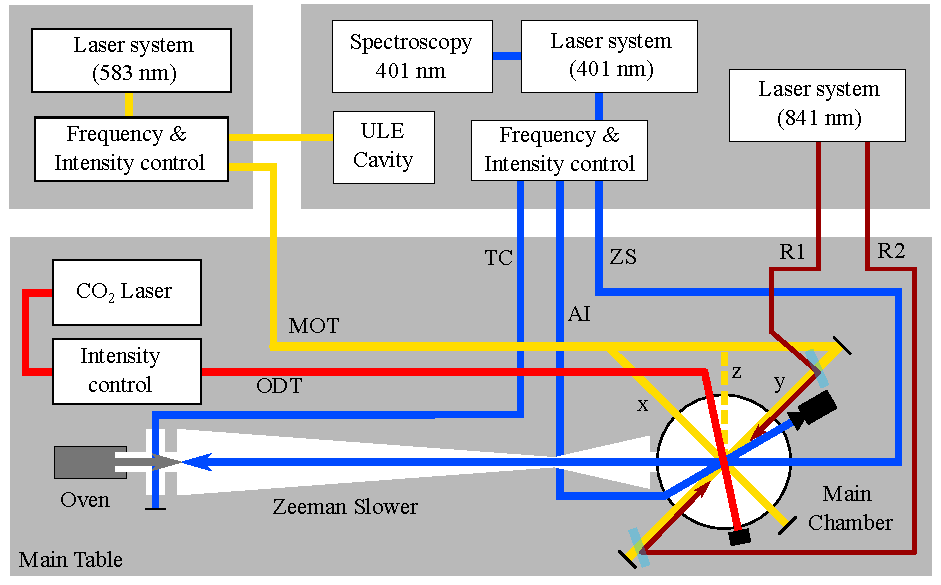
\includegraphics[width=1.\columnwidth]{table_set_up.pdf}
	\caption[Scheme of the experimental setup]{Scheme of the experimental setup. It is divided in three optical tables represented by gray areas. The 401nm laser system is used for the \acf{tc}, \acf{zs} and \acf{ai}. It is generated by a frequency doubled diode laser locked to a spectroscopic signal of the 401nm transition of $^{\text{168}}\text{Er}$. The 583nm laser system is used for the \acf{mot} and is frequency looked to an \acf{ule}. This trap uses 401nm laser beam in three spacial dimensions x, y and z. The $\text{CO}_{2}$ laser is used as main source of an \acf{odt}. The 841nm laser system is used to form the two lattice beams used for the Bragg scattering process which will be described in next Chapter.}\label{fig:table_set_up}. 
\end{figure}

Most of the laser systems in this experiment produce resonant light for the $^{\text{168}}\text{Er}$ atomic transitions. For this reason, these light sources are kept on different optical tables separated from the \ac{uhv} system. Thus, unwanted atom-light interaction that could damage the cooling capabilities of the experiment is reduced. This laser light is guided into the main table by using optical fibers that can be blocked and unblocked through the use of \acp{aom} before the fiber coupler. Allowing for a fast response time (typically a few microseconds) and better control of the experimental phases.

The different phases required to obtain an erbium \ac{bec} are chronologically very organized. There is almost no temporal overlay between phases. This allows for a very accurate description of the experiment by just explaining every procedure in a chronological order. In every cycle, the atoms start in the oven and pass through the \ac{tc} and \acf{zs} to reach the main chamber, where the \ac{mot}, \ac{odt} and evaporative cooling take place to generate the erbium \acl*{bec}.

\subsection{Oven}\label{subsec:oven}

The required first step to form an erbium \ac{bec} consist in transforming a solid state metal, with a high purity of erbium atoms (typically over 99\%), into an atomic beam. There are multiple reasons to why this is necessary. The main one being that it reduces the interaction between atoms and allows for laser cooling and trapping techniques. This will become more clear in the next experimental phases.

In order to produce an erbium beam, an oven of the type known as \Acf{dfc}\footnote{Model DFC-40-10-WK-2B by CreaTec Fischer \& Co. GmbH} is used, operating inside an \ac{uhv} chamber. The left side of Figure \ref{fig:experiment_scheme_1} shows a basic scheme of this device, which is divided into two tantalum wired cavities. The first one is called \Acf{ec} and contains the bulk metal of erbium, which is heated up to \SI{1200}{\degreeCelsius} and sublimated into gas. After this, the erbium gas is transferred through a \SI{3}{\centi\meter} pinhole into the second cavity of the \ac{dfc} known as \Acf{hl}. This last part of the oven is heated a \SI{100}{\degreeCelsius} higher than the \ac{ec} temperature to avoid condensation of material at the pinholes. Lastly, the erbium gas leaves the oven forming an atomic beam through a second pinhole that connects the \ac{hl} cavity with all the following experimental stages. In order to avoid the atomic beam from altering some of these sensitive experimental phases, the second pinhole is closed by a mechanical shutter at these moments. 

The speed at which the atoms are leaving the oven can be estimated in average with a parameter called \ac{rms} velocity $\bar{v}_{RMS}$. For the case of an ideal gas it has been obtained as \cite{Hansch1975}

\begin{equation}\label{eq:rms_velocity}
	\bar{v}_{RMS} = \sqrt{\frac{3 k_B T}{M}}
\end{equation}

This means that for a \ac{hl} temperature of \SI{1400}{\kelvin} the resulting \ac{rms} velocity of the erbium beam leaving the oven is approximately \SI{457}{\meter\per\second}.



\begin{figure}[!htbp]\centering
	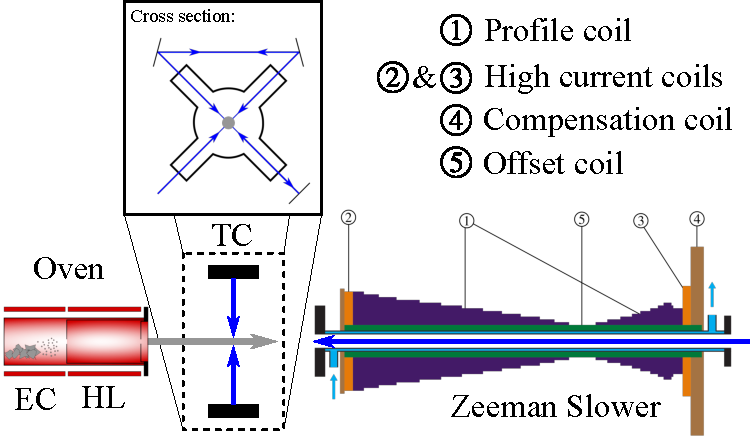
\includegraphics[width=1.\columnwidth]{experiment_scheme_1.pdf}
	\caption[Oven, \acl{tc} and \acl{zs} schemes]{Scheme of the oven, \acl{tc} and \acl{zs}. The atomic beam of erbium and the \SI{401}{\nano\meter} laser beam are represented by gray and blue arrows respectively. A cross section of the \acl{tc} can be seen inside a box. And the different coils used for the \acl{zs} are also represented.}\label{fig:experiment_scheme_1}
\end{figure}



\subsection{Transversal and Optical cooling}

An atomic beam produced by the \ac{dfc} oven presents two main problems: a poor collimation of the beam and a high speed of the erbium atoms forming the beam. These obstacles must be fixed before being able to trap the atoms into an atomic ensemble and form an erbium \ac{bec}. The main purpose of this \Acf{tc} phase is to solve the problem due to poor beam collimation. While the high atomic speed problem will be dealt with in the following \Acl{zs} section. However, these two phases are based in the same underlying physical principle, commonly known as Optical or Laser cooling. 

\subsubsection{Optical cooling}

This technique relies on the force applied on particles by red-detuned near resonant photons. From Equation \eqref{eq:rms_velocity}, it can be seen that the temperature of an ideal gas is proportional to its velocity. So this light-produced force, known as radiation pressure, can be used as a way to lower the temperature of an atomic gas simply by reducing its overall speed. To gain an insight into the physical model of this force, it is necessary to analyse a two-level atomic system  \cite{Metcalf1999}.

Due to this, an two level atom must be considered, which has a ground state $\ket{g}$, an excited state $\ket{e}$ and an energy difference between both states of $\Delta E = \hbar \omega_0$, here $\omega_0$ represents the atomic resonance frequency. The atom at rest can absorb a photon with resonant frequency $\omega_0$. Thus, transferring its energy $\hbar \omega_0$ and momentum $\vec{p}= \hbar \vec{k}$ to the atom. Where $\vec{k}$ represents the photon wave vector, such as for light with wavelength $\lambda$, the wave number results $|\vec{k}| = 2 \pi / \lambda$. According to which was the initial state of the atom before receiving the photon, it can relax into the ground state by spontaneous or by stimulated emission. The first case is produced when the atom was initially at the state $\ket{e}$, which makes the incoming photon trigger an relaxation into $\ket{g}$ of the atom. Resulting in the production of a second identical photon with the same frequency and direction than the triggering one. Because of this, the momentum transfer of the initial photon gets cancelled by the second one and therefore the effective momentum transferred to the atom adds up to zero. However, the second case of spontaneous emission results in a non-zero momentum transfer. Because in this case, the atom is initially in the ground state, allowing it to absorb the initial photon to get in the excited state. After a decay time $\tau$ the atom decays back to $\ket{g}$ and re-emits a second photon in a random direction. Due to the fact, that this photon is at average emitted isotropically in all directions, the momentum transfer produced by the second photon adds up to zero. Resulting in an effective momentum transfer of the atom equal to the initial momentum of the first photon.

In order to obtain an analytical analysis, the Bloch equations must be solved for a two level system. Resulting in the stationary solution for an occupation probability of the excited given by

\begin{equation}\label{eq:probablility_excited_state}
	\rho_{ee} = \frac{s_0/2}{1 + s_0 + \Big(\frac{2\delta}{\gamma}\Big)^2}
\end{equation}

Where $\gamma = 1/\tau$ is the decay rate, $\delta = \omega - \omega_0$ the detuning between laser light and atomic resonance  frequency and $s_0 = I / I_s$ the saturation parameter defined as the ratio of laser light intensity $I$ and saturation intensity $I_s = 2 \pi^2 \hbar c/ 3 \lambda^2 \tau$, with $\lambda$ the light wavelength and $c$ the speed of light. The radiation pressure force can be calculated using Equation  \eqref{eq:probablility_excited_state} as

\begin{equation}\label{eq:radiation_pressure_no_doppler}
	\vec{F} = \hbar \vec{k} \gamma \rho_{ee} = \hbar \vec{k} \gamma \frac{s_0/2}{1 + s_0 + \Big(\frac{2\delta}{\gamma}\Big)^2}
\end{equation}

However, this equation is only valid for a system of coordinates at rest with respect to the atom. This means that for an atom moving at a velocity $\vec{v}$, the light frequency received by the atom will be Doppler shifted an amount  $\Delta \omega_D = -\vec{k}\vec{v}$. By adapting Equation \eqref{eq:radiation_pressure_no_doppler} to the Doppler shift results

 \begin{equation}\label{eq:radiation_pressure}
 	\vec{F} = \frac{\hbar \vec{k} \gamma}{2} \frac{s_0}{1 + s_0 + \Big(\frac{2(\delta-\vec{k}\vec{v})}{\gamma}\Big)^2}
 \end{equation}

This equation for the radiation pressure suggests that a beam of atoms can be slowed down by a red-detuned ($\delta < 0$) counter-propagating optical beam. And therefore, the atomic beam temperature can decreases by following Equation \eqref{eq:rms_velocity}. However, this cooling process presents some limitations because of the spontaneous emission of the second photon. As already said, this spontaneous emission process has a vanishing momentum transfer. But its mean squared value does not vanish, thus heating up the atoms. For a limiting case in which this heating effect equals the optical cooling, an equilibrium temperature is reached known as Doppler limit or Doppler temperature, $T_D$.

\begin{equation}\label{eq:Doppler_limit}
	T_D = \frac{\hbar \gamma}{2 k_B}
\end{equation}

Which is a theoretical temperature limit for an ideal two levels atom \cite{Metcalf1999}. It can be seen from Equations \eqref{eq:radiation_pressure} and \eqref{eq:Doppler_limit}, that there must be a trade off in the experimental value for decay rate of the excited level $\gamma$. In order to achieve a strong enough value for the radiation pressure at the same time that a low enough Doppler temperature. There is however, the capability of cooling down further than the Doppler limit with the use of more refined techniques for multilevel atoms, such as the polarization gradient cooling approach \cite{Dalibard1989}. Nonetheless, for the case of complex multilevel elements like erbium, excited atoms may decay into intermediate states. This limits the cooling process and can suppress it almost completely, due to possible selection rules or high decay times in these intermediate states. If this is our case, the problematic state is commonly called Dark state. To solve this issue, additional pumping lasers or effectively closed transitions must be considered.

\subsubsection{\Acf{tc}}

Through the use of Optical cooling physical principles this experimental phase is used to collimate the atomic beam produced by the \ac{dfc} oven. In Figure \ref{fig:experiment_scheme_1}, a scheme and cross section of the \ac{tc} can be seen. The main objective is to increase the flux of atoms passing from \ac{dfc} to the initial part of the \ac{zs} aperture. To achieve this, a crossed optical beam of the red-detuned \SI{401}{\nano\meter} transition, transversal to the atomic beam, is used. As seen in the cross section scheme, the optical cross beam is overlaid with an ingoing and outgoing part. This results in four optical beams traversing the atomic beam in four perpendicular directions. This scheme together with the optical force described Equation \ref{eq:radiation_pressure} leads to radiation pressure acting towards the atomic beam centre, collimating it. Moreover, the high value for the decay rate of $\gamma = \SI{2.22e8}{\per\second}$ for the \SI{401}{\nano\meter} transition (see Table \ref{tab:Transitions}) makes the radiation pressure force considerably strong. In order to enhance the interaction between atomic and light beam, this last one has its shape widened elliptically with the mayor axis parallel to the atomic beam.


\subsection{\Acf{zs}}

As it has already been discussed in the previous section, the second problem that arises is the high speed at which the atomic beam is travelling. At the end of Section \ref{subsec:oven}, a calculation of the average speed of atoms leaving the oven resulted in approximately \SI{457}{\meter\per\second}. However, it has been estimated that the maximal trapping velocity is a few meters per second, for the specific \acl{mot} used in this experiment \cite{Ulitzsch2016}. The main objective of this experimental phase is to reduce the average atomic speed so that it is feasible to trap the atoms in an atomic ensemble. This requires another red-detuned laser beam from the \SI{401}{\nano\meter} transition moving in the opposite direction of the atomic beam. A counter-propagating optical beam transmits radiative pressure to the atomic beam as seen in Equation \eqref{eq:radiation_pressure}. However, as the atomic beam begins to be slowed down, the average velocity of the atoms $\vec{v}$ is reduced and the Doppler shift value $\Delta \omega_D = -\vec{k}\vec{v}$ in Equation \eqref{eq:radiation_pressure} also decreases. This results in a change of the resonance condition and suppression of the radiative pressure, which reduces the slowing effect of the atomic beam. In order to avoid this, the inner splinting of the atomic energy levels must be changed with the use of an spatially varying magnetic field. Thus, at the same time that the beam is being slowed down, the effective atomic resonance is being changed to match a reduction of the Doppler shift $\Delta \omega_D$. The atomic energy shift is affected by the position-dependent magnetic field $\vec{B}$, where the dominant effect is called Zeeman splitting $\Delta \omega_Z$, given by \cite{Zeeman1897}

\begin{equation}
	\Delta \omega_Z = \frac{\mu_{\text{eff}}}{\hbar} |\vec{B}|
\end{equation}

Where $\mu_{\text{eff}}$ represents the effective magnetic moment \cite{Metcalf1999}. By considering the desired case in which the Zeeman and Doppler shifts compensate each other $\omega_Z = -\omega_D$, and using also some basic kinematic theory. The required magnetic field can be obtained as a function of position $z$ at the axis in which the atomic beam is moving:

\begin{equation}\label{eq:magnetic_field_zeeman_slower}
	|\vec{B}(z)| = \frac{\hbar k}{\mu_{\text{eff}}}\sqrt{v_0^2 + 2 a(z-z_0)}
\end{equation}

With $a$ being the deceleration parameter, $v_0$ the maximal velocity at which the atoms can be slowed down and $z_0$ the spacial point where the atom deceleration begins. These types of magnetic fields can be shaped using coils with a spatial dependent number of wires, which is the case for a common \acf{zs} like the one used in this experiment. Figure \ref{fig:experiment_scheme_1} shows a scheme of the \ac{zs} with a counter propagating beam of \SI{401}{\nano\meter} transition providing the radiation pressure to the atomic beam and a group of five independent coils providing the magnetic field described by Equation \eqref{eq:magnetic_field_zeeman_slower}. For more details on the \ac{zs} experimental set-up and the description of these coils refer to \cite{Rehberger2013}.

\subsection{\Acf{mot}}

Once the atomic beam has passed the \ac{zs} and has been slowed down to a few meters per second, the erbium atoms enter the main \ac{uhv} chamber shown in Figure \ref{fig:main_chamber}. The next step requires trapping the atoms in a local region of the main chamber with the use of a \Acf{mot}. Thus, the atomic beam forms an ensemble of atoms with an even lower average velocity, which means a reduction in the erbium atoms temperature within the ensemble. 

\pagebreak

In this case, the \ac{mot} used consists of three pairs of counter-propagating laser beams red-detuned to the \SI{583}{\nano\meter} transition. Each of these beam pairs is perpendicular to the other two, forming three spatial axes inside the main chamber ($x$, $y$ and $z$) with an overlay region where the atomic ensemble will be made. In addition to this, two water cooled coils in an anti-Helmholtz configuration are required to create a quadrupole magnetic field, which is zero inside the overlaying region of the six laser beams. The result of this magneto-optical set up is the generation of a three dimensional spatially dependent restoring force, which binds the erbium atoms to remain inside the overlaying region. To have a physical interpretation of why this is happening, it is necessary to consider a two level atom located inside this region. The atom has a ground state $g$ with a total angular momentum quantum number of $J=0$ and an excited state $e$ with $J'=1$. Due to spatial symmetry and to simplify things even further, just effects in the $z$ axis will be considered. A scheme of this model can be observed in Figure \ref{fig:MOT_Energy}. Because of Zeeman splitting, the magnetic field $B_z = A z$ produced by the anti-Helmholtz coils at the $z$ direction, splits up the atomic states' degeneracies. Thus, for the ground state $m_g = 0$ because $J=0$ and there is no splitting, but for the excited state $m_e = [-1, 0, 1]$ because $J'=1$ splitting this state into three. The resulting force $\vec{F} = F \vec{e_z}$ being applied to an atom at a position $z'$ and a speed $\vec{v} = v \vec{e_z}$ comes from Equation \eqref{eq:radiation_pressure} applied in the two axial directions:

\begin{equation}\label{eq:MOT_force}
	\vec{F} = \frac{\hbar \vec{k} \gamma}{2} \frac{s_0}{1 + s_0 + \Big(\frac{2\delta_+}{\gamma}\Big)^2} - \frac{\hbar \vec{k} \gamma}{2} \frac{s_0}{1 + s_0 + \Big(\frac{2\delta_-}{\gamma}\Big)^2}
\end{equation}

Where:

\begin{equation}\label{eq:delta_plus_minus}
	\delta_\pm = \delta \mp \vec{k} \vec{v} \pm \frac{ \mu_{ \text{eff} } B_{z'} }{ \hbar }
\end{equation}

\begin{equation}\label{eq:mu_eff}
	\mu_{ \text{eff} } = \mu_B (g_e m_e - g_g m_g)
\end{equation}

With $\mu_B$ the Bohr magneton, $g_{g/e}$ the Landé factor and $\pm \vec{k} = \pm |k| \vec{e_z}$ the wave vector of both beams. As a result of this, the atom located in $z'$ will interact most likely with the light beam for which the detuning $\delta_+$ or $\delta_-$ is smaller. This means that an atom moving in any direction away from the \ac{mot} will absorb only photons from the optical beams that can push it towards the \ac{mot}'s centre. Because of the fact that erbium's \SI{583}{\nano\meter} transition has a narrow line-width of \SI{185.71}{\kilo\hertz} (see Table \ref{tab:Transitions}), the type of \ac{mot} used here is commonly known as a narrow-line \ac{mot}, which allows to achieve lower temperatures due to Equation \eqref{eq:Doppler_limit}. The experimental phase of the \ac{mot} can be divided into two main parts. The first one being known as the Loading phase, where the erbium atoms are collected from the \ac{zs}. And lastly, the Compressing phase, where the ensemble of atoms inside the \ac{mot} is compressed by detuning the lasers and magnetic fields. The result of this is a denser and more confined atomic cloud, which is useful for the \ac{odt} phase. Some typical temperatures achieved for erbium clouds trapped in the used \ac{mot} are in the \si{\micro\kelvin} regime. For a more in deep description of the underlying principles of \Aclp{mot}, or a characterization of the used set up, refer to \cite{Metcalf1999, Ulitzsch2016, Roell2016}. 

\pagebreak

\begin{figure}[!htbp]\centering
	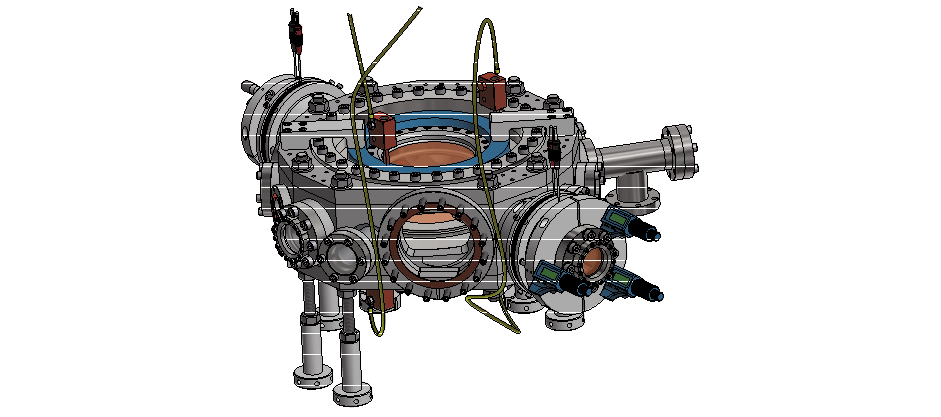
\includegraphics[width=1.\columnwidth]{main_chamber.pdf}
	\caption[Technical drawing of the main chamber]{Technical drawing of the main chamber. It has 17 viewports with different diameters and each one with anti-reflection coatings for the used laser transitions. The chamber also counts with a configuration of water cooled coils inside it, and some micrometer screws connected to lenses for collimation of the different laser beams passing through the ports. }\label{fig:main_chamber}
\end{figure}


\begin{figure}[!htbp]\centering
	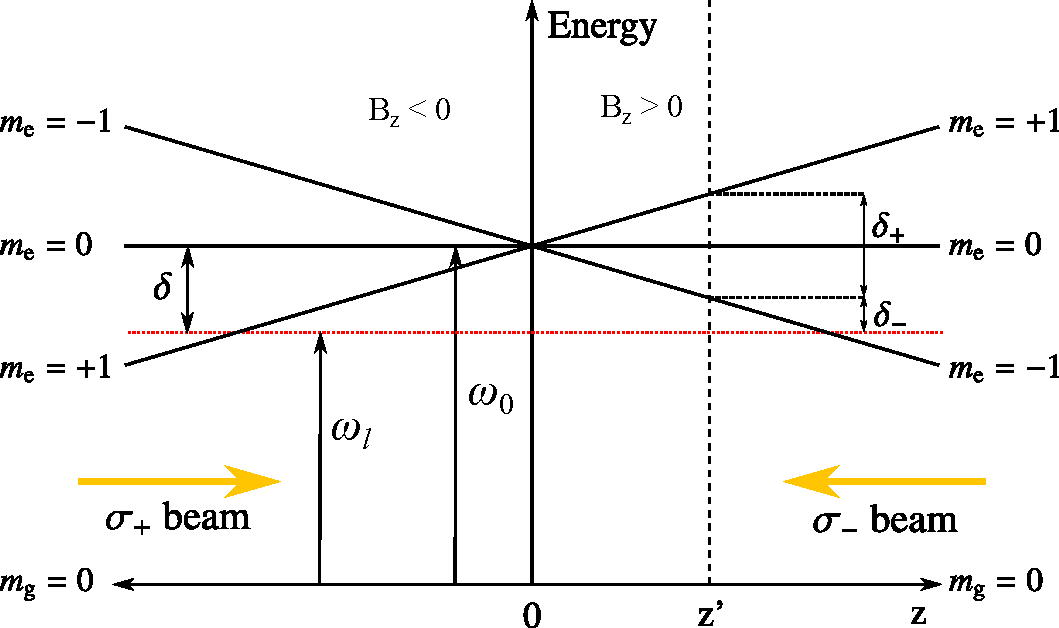
\includegraphics[width=0.9\columnwidth]{MOT_Energy.pdf}
	\caption[Atomic scheme of energies inside the \ac{mot} for a $J=0 \arrowvert J'=1$ transition in the z axis]{Atomic scheme of energies inside the \ac{mot} for a $J=0 \rightarrow J'=1$ transition in the z axis. It shows the Zeeman splinting of the excited state with $J'=1$ into three different states with $m_e = -1, 0, 1$, due to the quadrupole magnetic field produced by two coils in anti-Helmholtz configuration. A counter-propagating pair of circularly polarized laser beams is represented by two yellow arrows. They have a frequency $\omega_l$ illustrated in the energetic scheme by a red dashed line. These optical beams are red-detuned by $\delta = \omega_0 - \omega_l$, where $\omega_0$ is the erbium frequency of the \SI{583}{\nano\meter} transition. Figure modified from original in \cite{Metcalf1999}.}\label{fig:MOT_Energy}
\end{figure}

\subsection{\Acf{odt}}



%%% Local Variables: 
%%% mode: latex
%%% TeX-master: "Thesis"
%%% End: 